\documentclass[sts]{imsart}

%\usepackage{amsthm,amsmath,natbib}
%\RequirePackage[colorlinks,citecolor=blue,urlcolor=blue]{hyperref}

% put your definitions there:
%\startlocaldefs
%\endlocaldefs

\usepackage[author-year]{amsrefs}
\usepackage{bm,bbm}
\usepackage{siunitx}

\usepackage{amssymb}
\usepackage{enumerate}
\usepackage{color}
\usepackage{siunitx}

\usepackage{graphicx}
\graphicspath{{./Figures/}}

\begin{document}

\begin{frontmatter}

\title{Confidence Regions for Information-Theoretic Descriptors of Time Series}
\runtitle{Confidence Regions}

\author{\fnms{Marcelo} \snm{Queiroz}\corref{}\ead[label=e1]{marceloqgao@gmail.com}}
\and
\author{\fnms{Osvaldo A.} \snm{Rosso}\ead[label=e2]{oarosso@gmail.com}}
\and\\
\author{\fnms{Heitor S.} \snm{Ramos}\ead[label=e3]{heitor@laccan.ufal.br}}
\and
\author{\fnms{Christopher G.\ S.} \snm{Freitas}\ead[label=e6]{christopher@laccan.ufal.br}}
\and\\
\author{\fnms{Leonardo V.} \snm{Pereira}\ead[label=e4]{lviana@ic.ufal.br}}
\and
\author{\fnms{Alejandro C.} \snm{Frery}\ead[label=e5]{acfrery@laccan.ufal.br}}
\address{Av.\ Lourival Melo Mota, s/n\\
57072-900 Macei\'o, Brazil \printead{e1}}
\affiliation{Laborat\'orio de Computa\c c\~ao Cient\'ifica e An\'alise Num\'erica\\Universidade Federal de Alagoas}


\runauthor{M.\ Queiroz}

\begin{abstract}
The \citeauthor{PermutationEntropyBandtPompe} methodology has been used with success in time series analysis.
It consists in computing Information-Theoretic descriptors, from a histogram of ordinal patterns, which lie in a 2D manifold: the Entropy-Complexity plane.
So far, the analysis of the dynamics underlying the time series has been performed using two reference points: those corresponding to a deterministic and to white noise time series.
In this paper we provide confidence regions for white and $f^{-k}$ noise models.
These regions allow testing whether a sequence belongs to one of these models.
\end{abstract}

\begin{keyword}[class=MSC]
\kwd[Primary ]{37M10}
\kwd[; secondary ]{68Q30}
\end{keyword}

\begin{keyword}
\kwd{Nonparametric time series analysis}
\kwd{ordinal patterns}
\kwd{Information Theory}
\end{keyword}

\end{frontmatter}

\section{Introduction}\label{Sec:Intro}

Time Series carry valuable information about the system which produces the data.
Their analysis is usually based on two approaches \cite{TimeSeriesAnalysisCryerChan}: in the (natural) time and transformed domains (for instance, frequency and wavelet).

A new methodology was proposed by \citeauthor{PermutationEntropyBandtPompe}~\ycite{PermutationEntropyBandtPompe}.
Their approach is nonparametric and based on Information Theory descriptors.
The time series is transformed into ordinal patterns, with which a histogram is formed.
This approach is less sensitive to outliers, and as it does not rely on any model it can be applied to a variety of situations.

Each time series is described by a point in a manifold of $\mathbbm R^2$, namely the Entropy-Complexity plane.
Two points are well known in this plane: those of white noise and of a completely deterministic sequence.

The Band and Pompe methodology and its variants have been successfully used in the analysis of many types of dynamics.
To date, the original work has received around \num{1000} cites, according to the Journal of Citation Records.

A few highlights of the related literature are the following.
\citeauthor{RandomNumberGeneratorsCausality}~\ycite{RandomNumberGeneratorsCausality}
show that the Entropy-Complexity plane ($H\times C$) is a good indicator of the results of Diehard tests for pseudorandom number generators.
\citeauthor{GeneralizedStatisticalComplexityMeasuresGeometricalAnalyticalProperties}~\ycite{GeneralizedStatisticalComplexityMeasuresGeometricalAnalyticalProperties} analyze the logistic chaotic map and discuss the boundaries of the $H\times C$ plane.
\citeauthor{EEGAnalysisWaveletInformationTools}~\ycite{EEGAnalysisWaveletInformationTools} study electroencephalography signals using wavelet decompositions and the $H\times C$ plane.
\citeauthor{De_Micco_2008}~\ycite{De_Micco_2008} assess ways of improving pseudorandom sequences by their representation in this plane.
\citeauthor{De_Micco_2009}~\ycite{De_Micco_2009} study chaotic components in pseudorandom numbers generators.
\citeauthor{ComplexNetworksEvolution}~\ycite{ComplexNetworksEvolution} analyze the evolution of dynamic networks by trajectories in the $H\times C$ plane.
\citeauthor{DistinguishingChaoticStochasticDynamicsTimeSeriesMultiscaleSymbolicApproach}~\ycite{DistinguishingChaoticStochasticDynamicsTimeSeriesMultiscaleSymbolicApproach} use a multiscale approach to analyze the interplay between chaotic and stochastic dynamics.
\citeauthor{StructuralChangesDataCommunicationWSN}~\ycite{StructuralChangesDataCommunicationWSN} employ Information-Theoretic measures to describe the evolution of wireless sensors networks.
\citeauthor{DistinguishingNoiseFromChaos}~\ycite{DistinguishingNoiseFromChaos} tackle the often hard problem of distinguishing chaos and noise.
\citeauthor{CharacterizationVehicleBehaviorInformationTheory}~\ycite{CharacterizationVehicleBehaviorInformationTheory} describe the behavior of vehicles as a function of the topology of cities.
\citeauthor{LiborInvisibleHand}~\ycite{LiborInvisibleHand} identify spurious interventions in the Libor market using the $H\times C$ plane representation.
\citeauthor{DiagnosingDynamicsObservedSimulatedEcosystem}~\ycite{DiagnosingDynamicsObservedSimulatedEcosystem} use this tool to analyze time series from natural phenomena.
\citeauthor{InformationTheoryPerspectiveNetworkRobustness}~\ycite{InformationTheoryPerspectiveNetworkRobustness} check the effect of attacks to complex networks by the displacement of their points in the $H\times C$ plane.
\citeauthor{ClassificationVerificationOnlineHandwrittenSignatures}~\ycite{ClassificationVerificationOnlineHandwrittenSignatures} show that these descriptors are able to classify and verify online signatures.
\citeauthor{CharacterizationElectricLoadInformationTheoryQuantifiers}~\ycite{CharacterizationElectricLoadInformationTheoryQuantifiers}
show that Information-Theoretic descriptors are able to characterize types of electric appliances by records of their energy consumption.

In spite of these and many other applications, only recently \cites{OrdinalPatternProbabilities,NewPermutationEntropy} the literature has started paying attention to the inherent randomness of points in the $H\times C$ plane.
The knowledge of the expected variability of such points according to the underlying dynamics would allow making hypotheses tests to a variety of models.

This paper advances the state-of-the-art by providing confidence regions for points in the $H\times C$ plane for a diversity of situations of interest.
Such regions are obtained using a Monte Carlo approach.
The input is a sequence of actual random observations generated by a physical procedure.

Section~\ref{Sec:Intro} introduces the elements of the study (the Bandt and Pompe methodology, the random deviates and models).
The confidence regions are presented in Section~\ref{Sec:Results}, and the conclusions are discussed in Section~\ref{Sec:Conclusions}.


\section{Methodology}\label{Sec:Method}

\subsection{The Bandt and Pompe Methodology}

Let ${\mathcal X} \equiv \{x_t\}_{t=1}^{T}$ be a real valued time series of length $T$, without ties. 
As stated by \citeauthor{PermutationEntropyBandtPompe}~\ycite{PermutationEntropyBandtPompe} in their seminal work:  
\begin{quote}
``If the $\{x_t\}_{t=1}^{T}$ attain infinitely many values, it is common to replace them by a symbol sequence 
$\Pi \equiv \{\pi_j\}$ with finitely many symbols, and calculate source entropy from it".
\end{quote}
Also, as stressed by these authors, 
\begin{quote}
``The corresponding symbol sequence must come 
naturally from the $\{x_t\}_{t=1}^{T}$ without former model assumptions".
\end{quote}

Let ${\mathfrak A}_{D}$ (with $D \geq 2$ and $D \in {\Bbb Z}$) be the symmetric group of order $D!$ formed by all 
possible permutation of order $D$, and the symbol component vector 
${\bm \pi}^{(D)} = (\pi_1, \pi_2, \dots, \pi_D)$ so every element ${\bm \pi}^{(D)}$ is unique 
($\pi_j \neq \pi_k~\forall~j \neq k$). 
Consider for the time series ${\mathcal X} \equiv \{x_t\}_{t=1}^{T}$ its time delay embedding representation,
with embedding dimension $D \geq 2$ ($D \in {\Bbb Z}$) and time delay $\tau \geq 1$ ($\tau \in {\Bbb Z}$, also called ``embedding time''):
\begin{equation} 
\label{eq:time-delay}
{\mathbf X}^{(D,\tau)}_t ~=~( x_t,x_{t+\tau},\dots,x_{t+(D-1)\tau} ) \ ,
\end{equation} 
for $t = 1,2,\dots,N$ with $N = T-(D-1) \tau$.
Then the vector ${\mathbf X}^{(D,\tau)}_t$ can be mapped to a symbol vector ${\bm \pi}^{(D)} \in {\mathfrak A}_{D}$. 
This mapping should be defined in a way that preserves the desired relation between the elements 
$x_t  \in {\mathbf X}^{(D,\tau)}_t$, and all $t \in T$ that share this pattern (also called motif) have to mapped to the same 
${\bm \pi}^{(D)}$. 
The two most frequent ways to define the mapping ${\mathbf X}^{(D,\tau)} \mapsto {\bm \pi}^{(D)}$ are:  
\begin{enumerate}[a)]
\item ordering the ranks of the $x_t \in {\mathbf X}^{(D,\tau)}$ in chronological order 
       (\textit{Rank Permutation}) or,
\item ordering the time indexes according to the ranks of $x_t \in {\mathbf X}^{(D,\tau)}$  
       (\textit{Chronological Index Permutation});
\end{enumerate}
       see details in \citeauthor{BPRepeatedValuesChaos}~\ycite{BPRepeatedValuesChaos}.
Without loss of generality, in the following we will only use the latter.



Consider, for instance, the time series $\mathcal X = (1.8, 1.2, 3.2, 4.8, 4.2, 4.5, 2.3, 3.7, 1.2, .5)$ depicted in Fig.~\ref{Fig:IntroBP}.
Assume we are using patterns of length $D=5$ with unitary time lag $\tau=1$.
The code associated to $\mathbf X_{3}^{(5,1)}=(x_3,\dots,x_7)=(3.2, 4.8, 4.2, 4.5, 2.3)$, shown in black, is formed by the indexes in $\bm\pi^{(5)}=(1,2,3,4,5)$ which sort the elements of $\mathbf X_{3}^{(5,1)}$ in increasing order: $51342$.
With this, $\widetilde{\pi}^{(5)} = 51342$, and we increase the counting related to this motif in the histogram of all possible patterns of size $D=5$.

The dash-dot line in Fig.~\ref{Fig:IntroBP} illustrates $\mathbf X_{1}^{(5,2)}$, i.e. the sequence of length $D=5$ starting at $x_1$ with lag $\tau=2$.
In this case, $\mathbf X_{1}^{(5,2)}= (1.8, 3.2, 4.2, 2.3, 1.2)$, and the corresponding motif is $\widetilde{\pi}^{(5)}=51423$.

\begin{figure}[hbt]
\centering
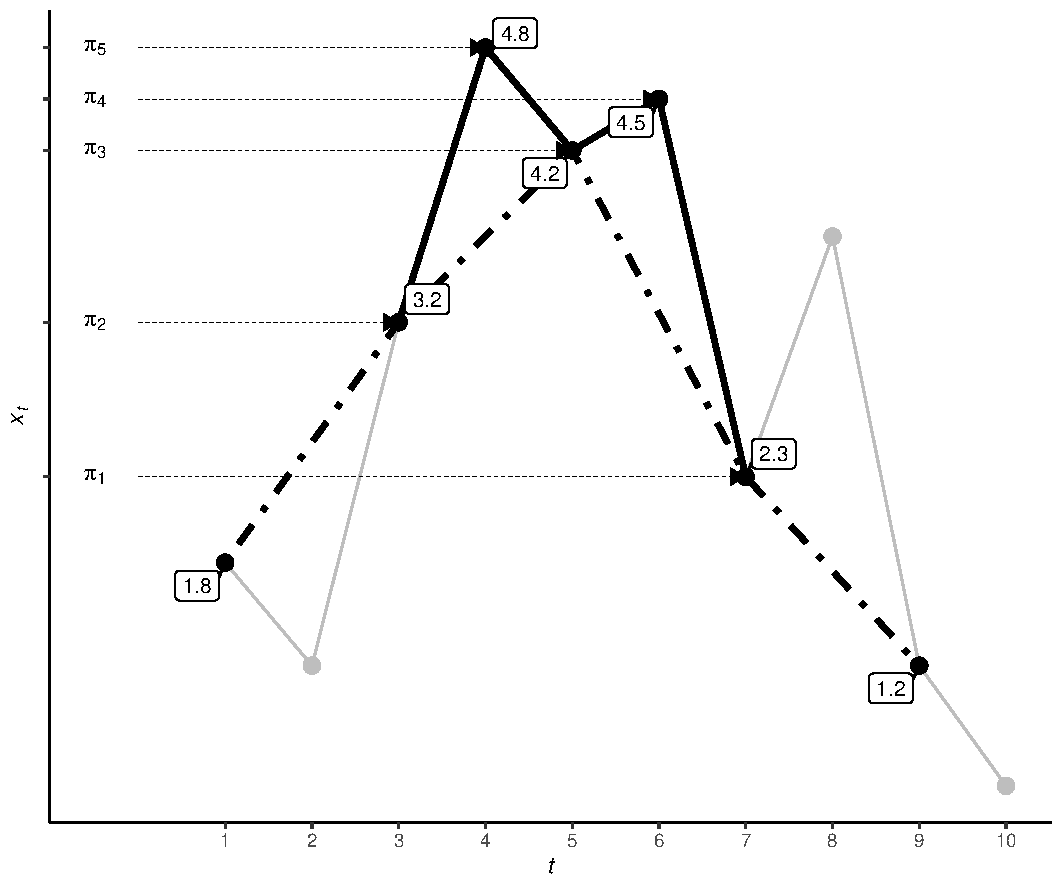
\includegraphics[width=.7\linewidth]{IntroBP}
\caption{Illustration of the Bandt and Pompe coding\label{Fig:IntroBP}}
\end{figure}

\subsection{The Entropy-Complexity Plane}

\textcolor{red}{Dar intui\c c\~ao sobre onde devem cair os pontos}

%
%Plano con: ruido k: 0, 0.5, 1, 1.5, 2., 2.5, 3
%Mapa logístico: r= 4, 3.6
%Monotónica creciente
%Periódica


\subsection{Random Deviates and Models}

\textcolor{red}{Gerador}

\textcolor{red}{Modelo $f^{-k}$}

\section{Results}\label{Sec:Results}

We employed the following factors in this study:
\begin{itemize}
\item Time series length $T\in\mathcal T=\{10^3,10^4, \num[scientific-notation=true]{5 e4}, \num[scientific-notation=true]{e5}, \num[scientific-notation=true]{5 e5}\}$,
\item Embedding dimension $D\in\mathcal D=\{3, 4, 5, 6\}$, and
\item Exponent of the $f^{-k}$ noise $k\in\mathcal K=\{0, 0.1, 0.5, 1, 1.5, 2\}$.
\end{itemize}
The only time delay we report is $\tau=1$.
We repeated the experiments for time lags $\tau=\{10,30,50\}$, and no significant differences were observed.
We obtained $1000$ independent series for each point in the factors set $\mathcal T\times \mathcal D\times \mathcal K$.

\textcolor{red}{An\'alise descritiva: alguns pontos de $\Theta$ representativos:} 
% k=0 white
% k=1 pink
% k=2 brown
% T = 1000, T = 5 10^5
% D= 3, D = 6

\textcolor{red}{Justificar an\'alise 1D}

\textcolor{red}{Intervalos de confian\c ca}

The data generation and analyses were performed using the \texttt R platform \cite{Rmanual} v.~3.4.4.
We used the \texttt{ggplot2} library \cite{ggplot2Wickman} for generating the plots.

\section{Conclusions}\label{Sec:Conclusions}

\bibliography{../Texto/references}

\end{document}
